\scanpage{50}

U N I V E R S I T E\par
DES SCIENCES ET TECHNIQUES\par
DU LANGUEDOC\par
------------\par
AMC/GJ

Montpellier, le 5 Juin 1975

\uline{Diffusion} : Liste A\par
N° 3510

\uline{AVIS DE SOUTENANCE D'UNE THESE DE DOCTORAT DE}\par
\uline{SPECIALITE : MATHEMATIQUES APPLIQUEES}

\uline{Nom et prénom du candidat} : NANARD Marc

\uline{Titre de la thèse} : L'influence de l'agencement des E.S. sur les performances
d'un système d'exploitation.

\uline{Date, heure et lieu de soutenance prévus} : 16 Juin 1975 à 10 heures\par
Salle de Cours n° 9, U.S.T.L.

\uline{Nom du Directeur de thèse} : J. FALGUEIRETTES

\uline{Désignation du laboratoire où la thèse est préparée} :\par
Centre de Recherche en Informatique et Gestion.

\uline{Analyse de l'ouvrage} : On étudie l'influence de l'organisation des entrées
sorties sur le comportement du système. On examine en particulier le problème
du fonctionnement parallèle de l'U.C. et des canaux et le problème des conflits
d'accès disque. Les modèles proposés sont appliqués à un exemple concret.

\uline{Durée approximative des recherches ayant abouti à la thèse} : 2 ans 1/2

\uline{Composition du jury proposé} :\par
\begin{tabular}{l}J. FALGUEIRETTES\\Y. ESCOUFIER\\J.P. VERJUS\\C. KAISER\end{tabular}

LE SECRETAIRE GENERAL,

\unsure{E. Siau}
\figure{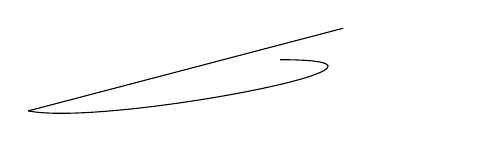
\begin{tikzpicture}[x=1cm,y=1cm]
\draw(0,0)--(4,1.05);\draw(0,0)..controls(1,-.2)and(5.4,.65)..(3.2,.65);
\end{tikzpicture}}
\uline{E. SIAU}

\begin{tabular}{ll}
MR\quad LE PROFESSEUR GROTHENDIECK A.&\\[1em]
MATHEMATIQUES&5-856
\end{tabular}

\mspage{49}
